\cleardoublepage

\chapter{Resultados}
\label{makereference7}

Los resultados de este apartado se basan en la exploración tipo Grid descrita en el apartado anterior. Los datos utilizados en esta exploración han sido los proporcionados por InfoRiego entre el 1 de enero de 2015 hasta el 31 de diciembre del 2015.

Para llevar a cabo el entrenamiento anterior, y poder obtener una métrica con la que evaluarlo, es necesario realizar una división del conjunto de datos en dos para cada prueba. Un conjunto para entrenar el modelo y otro para comprobar la precisión de este. Es importante que estos dos conjuntos sean complementarios ya que el modelo entrenado no debe conocer ningún dato del conjunto de test o el entrenamiento se vería alterado por conocer de antemano los datos a predecir.

El tamaño de cada conjunto es también un hecho relevante ya que con un conjunto de datos muy pequeño para el entrenamiento, la predicción sería dificilmente alcanzable con éxito y con un conjunto muy grande, habría pocos datos para probar que el modelo es fiable. Una división típica es dividir el conjunto de datos en 70/30, es decir, 70\% de los datos para entrenamiento y 30\% para comprobación. En este se ha utilizado una división 25/75 que es la utilizada por defecto por el grid search de SciKitLean.

Para poder analizar los resultados, la prueba anterior proporciona distintas métricas para medir la calidad del modelo. La implementación de GridSearch utilizada (librería de scikit-learn) pretende dar una misma interfaz para utilizar esta técnica con distintos algoritmos, por lo tanto, los resultados que se obtienen con ellos también tienen una misma forma de nombrar las métricas para todos.

Sin embargo, aunque en los ficheros de resultados aparezcan los mismos nombres para medir los resultados, el significado de estos es distinto dependiendo del modelo seleccionado. En los distintos apartados dedicados a cada uno de estos modelos se explicará el significado de sus métricas.

Junto con las métricas de calidad del modelo entrenado aparecen los parámetros necesarios para obtener dicho modelo. Tanto los parámetros específicos de cada modelo como el número de instantes anteriores utilizados (``k'') o la distancia a la predicción.

A la distancia a la predicción la llamaremos ``horizonte de predicción'' y especifica la diferencia entre la hora a la que se realiza la predicción y la hora a la que se quiere predecir entre el intervalo de medida (30 minutos para estos datos). Aunque se haya probado con varios horizontes, el que más nos interesa es ``2'', que indica una predicción a una hora.

Se han realizado tres conjuntos de pruebas, una por cada algoritmo predictivo estudiado. A continuación se analizan los resultados para cada uno de estos algoritmos.

\section{Regresión Lineal}
\label{makereference7.1}
Los parámetros suministrados a GridSearch para realizar el entrenamiento con este modelo son los siguientes:

\begin{itemize}
\item Inicio: 01-01-2015
\item Fin: 31-12-2015
\item k: 2, 3, 4, 5
\item Horizonte de predicción: 2, 3, 4, 5, 6, 7
\item fit\_intercept: true, false
\item copy\_X: true, false 
\end{itemize}

Grid serach estudiará los resultados para todas las combinaciones posibles.

De los resultados obtenidos para este algoritmo mostrados en la figura \ref{resultado_linear}, la columna ``mean'' nos indican el \(R^{2}\) obtenido. \(R^{2}\) es el coeficiente de correlación y, en regresión lineal, es el cuadrado del \textit{coeficiente de correlación de Pearson}. Se calcula dividiendo el cuadrado de la covarianza del conjunto de datos reales y los predichos entre el producto de los cuadrados de la desviación típica de cada conjunto. Expresa la calidad de la predicción del modelo entre 0 y 1.

\begin{figure}[htb]
	\begin{center}
		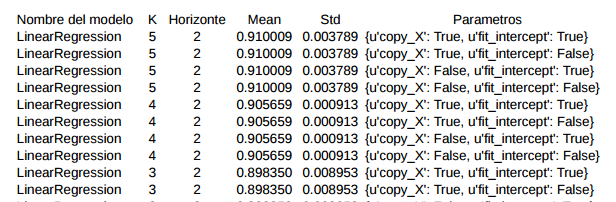
\includegraphics[width=14cm]{figures/resultado_linear.png}
		\caption{Resultado Regresión Lineal \label{resultado_linear}}
	\end{center}
\end{figure}

Los datos se muestran ordenados por la columna ``mean'' siendo así el primero de estos registros el que más coeficiente de correlación obtiene con un coeficiente de correlación de 0.910009.

Como se puede observar en la figura \ref{resultado_linear}, el modelo obtenido con mejor coeficiente de correlación tiene la siguiente configuración:

\begin{itemize}
\item Inicio: 01-01-2015
\item Fin: 31-12-2015
\item k: 5
\item Horizonte: 2
\item copy\_X: true
\item fit\_intercept: True
\end{itemize}

En el capítulo \ref{Appendix:Key1} (Anexo: Gráficas Regresión Lineal), se muestran distintas gráficas con la radiación de este modelo durante varios días del año, la predicción que obtenemos con el modelo obtenido con mayor coeficiente de correlación y el modelo conservador.

Este ``modelo conservador'' expresa una predicción de la radiación que se realiza asumiendo que en el instante \emph{t+1} la radiación será la misma que la observada en el instante \emph{t}.
El objetivo de este proyecto es superar, como mínimo este modelo conservador.

Junto a la leyenda de nuestro modelo y del modelo conservador, encontramos las siglas ``MAE'' (Mean Absolute Error), que es la media de las diferencias entre una radiación real y su predicción  en valor absoluto. Esto nos permite conocer la media del error expresado en la misma unidad que la radiación (W / \(m^2\)).

Como vistazo general, podemos observar que en todas las gráficas de resultados de regresión lineal, nuestro modelo obtiene un MAE mucho menor que el modelo conservador. Esto implica que nuestro modelo Regresión Lineal se ajusta mejor a la realidad.

En los días de primavera obtenemos los mejores resultados, en especial en las horas centrales del día. Quizá esto se deba a que la temperatura a estas horas es más estable que en el amanecer o atardecer.

Los días de verano e invierno, es dónde la diferencia de MAEs con respecto al modelo conservador es algo menor. Por lo que nuestra predicción sería levemente más acertada que dicho modelo.

\section{SVR}
\label{makereference7.2}

Para la exploración del modelo SVR usamos los siguientes parámetros:

\begin{itemize}
\item Inicio: 01-01-2015
\item Fin: 31-12-2015
\item k: 2, 3, 4, 5
\item Horizonte de predicción: 2, 3, 4, 5, 6, 7
\item C: 1, 10, 100, 1000
\item gamma: 0.001, 0.0001
\item kernel: linear, rbf 
\end{itemize}

En los resultados de la exploración mostrados en la figura \ref{resultado_svr}, la columna ``mean'' utiliza la misma métrica que la vista en el apartado anterior. Esto es porque ambas son regresiones y esta es muy utilizada en ese caso.

\begin{figure}[htb]
	\begin{center}
		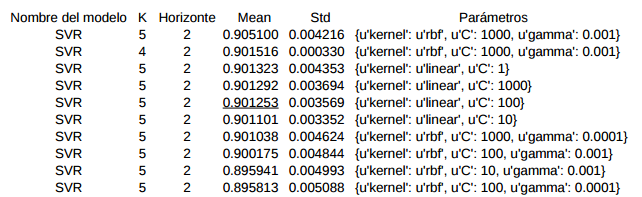
\includegraphics[width=14cm]{figures/resultado_svr.png}
		\caption{Resultado Regresión Lineal \label{resultado_svr}}
	\end{center}
\end{figure}

La figura \ref{resultado_svr} muestra el modelo obtenido con mejor coeficiente de correlación (0.905100) y su configuración:

\begin{itemize}
\item Inicio: 01-01-2015
\item Fin: 31-12-2015
\item k: 5
\item Horizonte de predicción: 2
\item C: 1000
\item gamma: 0.0001
\item kernel: rbf 
\end{itemize}

En el capítulo \ref{Appendix:Key2} (Anexo: Gráficas SVR) podemos observar varias gráficas para distintos días del año con la predicción obtenida con este modelo frente a la radiación real y al modelo conservador.

En los días de invierno, obtenemos un mejor MAE que el modelo conservador. Podemos observar que en las horas centrales del día es cuando mejor se ajusta, pero no tanto como primavera u otoño. Cuando peor se ajusta es en las primeras horas del día, en el amanecer.

En los días de las estaciones de primavera y otoño, nuestro modelo SVR obtiene una mayor diferencia respecto al MAE conservador, siendo mucho menor. Así podemos concluir, que en estas estaciones, quizá, es cuando mejor precisión obtenemos con nuestro modelo.

En los días de verano, podemos observar que nuestro modelo es cuando menor precisión tiene con respecto a la realidad. Siendo así, la única estación del año en la que el modelo conservador tiene un mejor MAE.

\section{Redes Neuronales}
\label{makereference7.3}

A continuación se indica los distintos parámetros con los que se ha explorado el modelo:

\begin{itemize}
\item Inicio: 01-01-2015
\item Fin: 31-12-2015
\item k: 2, 3, 4, 5
\item Horizonte de predicción: 2, 3, 4, 5, 6, 7
\item solver: lbfgs, sgd
\item hidden\_layers: (5, 2), (5, 3), (5, 4)
\item ramdon\_state: 1, 2
\end{itemize}

En este caso, la métrica utilizada para determinar la calidad del modelo ha sido ``accuracy'' (en español, exactitud). Es una métrica muy utilizada en clasificadores que indica el porcentaje de predicciones clasificadas correctamente.

\begin{figure}[htb]
	\begin{center}
		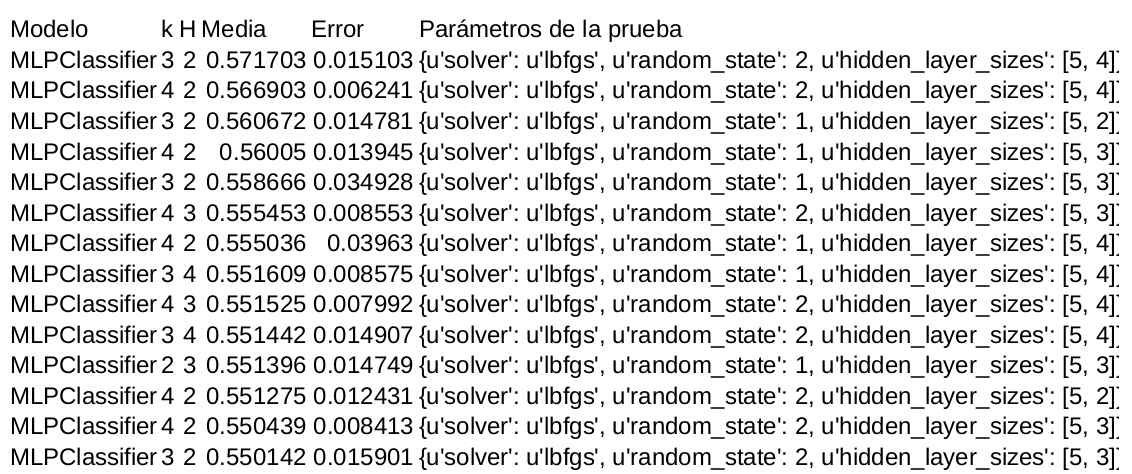
\includegraphics[width=17cm]{figures/resultado_mlp.png}
		\caption{Resultado redes neuronales \label{resultado_mlp}}
	\end{center}
\end{figure}

En la figura \ref{resultado_mlp} podemos ver los resultados del grid search para Redes Neuronales. La configuración del modelo con mayor ``accuracy'' obtenido es la siguiente:

\begin{itemize}
\item Inicio: 01-01-2015
\item Fin: 31-12-2015
\item k: 3
\item Horizonte de predicción: 2
\item solver: lbfgs
\item hidden\_layers: (5, 4)
\item ramdon\_state: 2
\end{itemize}

En el capítulo \ref{Appendix:Key3} tenemos distintas gráficas con la predicción realizada por este modelo, la radiación real y la predicción del modelo conservador para distintos días del año 2016.

Las conclusiones finales con nuestro modelo de redes neuronales es que hay que seguir investigando dicho modelo y sus parámetros. Obtenemos un ``accuracy'' o acierto del 0\%. Por lo que no hay mucho más que decir.